\documentclass[a4paper,10pt]{article}
\usepackage{graphicx}
\usepackage[pdfborder={0 0 0}]{hyperref}
\title{ Student Project 2017 \\ CalTech101 Image Classification}
\author{David Schulte, Hannes Martinke, Martin Zettwitz}

\begin{document}
\maketitle

\section{Introduction}
The classification of arbitrary pictures is an actual very hard task for image analysts, because the machine learning methods are difficult to use with the high number of pixel features in an image.
The task of the project is to classify the \emph{CalTech 101} dataset by using different feature selection and classifying approaches. 
The dataset contains images of 101 different categories. We had to achieve an accuracy of 10~\% with a 10-Fold cross validation.

\paragraph{Programming Environment}
Our classification approach is implemented in C++ with the use of \emph{Opencv} and \emph{dlib}.
\emph{Opencv} and \emph{dlib} are open source libraries for computer vision and machine learning tasks. 
Our first approaches were an implementation in \emph{Opencv}, because of some missing algorithm for the classification step in the library, we added the \emph{dlib} to combine both libraries.
The workflow of our procedure is illustrated in \autoref{fig:workflow} and consists of the following four steps: preprocessing, features generation, training, validation.
The steps will be explained in the next sections.

\begin{figure}[htb]
\centering
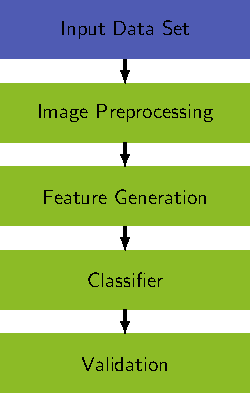
\includegraphics[scale=0.7]{images/Workflow.pdf}
\caption{Our worklow for the image classification. We organized the input data sets and prepared each image for the subsequent feature generation.
This features are used to train the classifier. The validation is performed in the next step to evaluate the classification results.}
\label{fig:workflow}
\end{figure}

\section{Preprocessing}
\label{sec:preprocessing}
Several images in the \emph{CalTech 101} dataset exist in different image sizes. 
This results in different lengths of the feature vectors within the feature generation.
To avoid this problem and we resized each image in the data set to 64x64, respectively 128x128.
An additional reason for the resizing is the computation time of the feature generator and the training. 
We tried to get a good trade-off between accuracy and computation time.
\begin{figure}[ht]
\centering
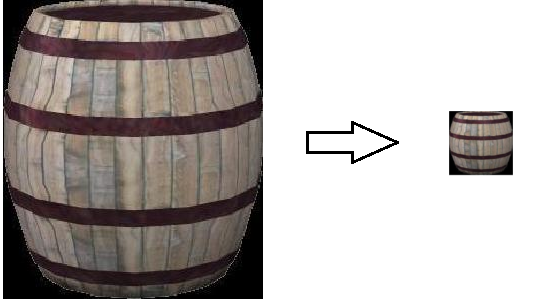
\includegraphics[scale=0.5]{images/preprocessing.png}
\caption{Illustration of the image re-sampling with an example image of a barrel.}
\label{fig:resize}
\end{figure}

\section{Features}
\subsection{Feature Generation}

We used the Histogram-of-Gradient~(HOG) \emph{INSERT PAPER} feature descriptor as it is a powerful technique to describe images independent of the lighting conditions. 
The Image is split into overlapping cells. The edges (defined by gradients) are assigned into different bins (uniformly distributed directions).
Because of the input image size it is necessary to choose a cell size to the power of two. 
We tested the cell size with 8, 16 and 32 for feature generation with a padding of 1.
We used the features extracting algorithm of \emph{dlib}, which calculates a 31 dimensional feature vector for each cell.
Two example images with the different parameters are shown in figure \emph{...}


\subsection{Feature Reduction}

The calculated features can be reduced by using for example principle component analysis(PCA) or other techniques.
In our approach an feature reduction is served by re-sampling the images in the preprocessing step (recall \autoref{sec:preprocessing}).
With the limitation of the pixel matrix and the use of HOG Features the length of the feature vector is equalized for each sample.

\section{Classifiers}

After generating the feature vectors for each sample, the samples of each class must be trained, followed by testing to evaluate the accuracy of the whole classification approach. 
Therefore we implement two different classifiers. 

\paragraph{AdaBoost}
Adaptive Boosting \emph{INSERT PAPER Fre95} is machine learning approach, that is based on so called \textit{weak classifiers} that will form a \textit{strong classifier}. Each weak classifier is assigned to randomly generated feature, its prediction is just slightly better than random guessing. The power of the technique is done by combining the best $n$ weak classifiers to a strong classifier as a powerful descriptor. The weak classifiers are trained by supervised learning where each weak classifier predicts the samples. Based on that prediction the error rate is assigned to the individual weak classifier. Additionally each sample is weighted by its significance (error rate of the best weak classifier) to emphasize unseen and hard to predict training data. Based on that significance weight and the error rate of a weak classifier, each weak classifier that is combined to the strong one is weighted, too.
\paragraph{SVM}
A Support-Vector-Machine basically tries to define a hyperplane to distinguish between classes in datasets. Therefore support-vectors are created, that maximizes the distance between the closest points of (two) classes. To separate between non-linear datasets, the feature space is mapped onto an higher dimensional space, using a kernel, where a linear separation is possible. Mapped back onto the original feature space one obtains the hyperplane. This way even initial high dimensional datasets can be distinguished. To reduce the computational effort one uses Mercer's theorem, that only implicitly computes the data in the higher dimension, but instead uses a kernel function. Well used kernels are polynomial kernels and radial-base-function kernels like Gaussian. We used a Nu-SVM with parameter $Nu$ as constrain for the hyperplane in a range of $[0,1]$. We tested several values by iteratively increasing $Nu$ until the classification error was minimized with a $Nu$-value of $0.00511$ 

\section{Training and Validation}
To train and validate our approach we used a 10-fold cross validation. 
This method divides the data set in 10 subsets of equal size. 9 folds will be trained and the last one is for testing of the classifier.
This is an iterative process and will be performed using permutation until each fold was tested.
To observe the process, we counted the number of predictions and assigned the positive predictions to the predicted class.
\section{Results}
Matrix + Conclusion 

\end{document}

\grid
\grid
